\setcounter{section}{5}
\setcounter{subsection}{11} % 5.12
\subsection{TCP-Retransmission-Timer}

Siehe Tabelle~\ref{tab:5.12} und
Abbildungen~\ref{fig:5.12.c.Zeit-SampleRTT}, \ref{fig:5.12.c.Zeit-EstimatedRTT}, \ref{fig:5.12.c.Zeit-Timeout-Original} und \ref{fig:5.12.c.Zeit-Timeout-Jacobsen}

\FloatBarrier

\begin{table}[p]
    \centering
    \import{./assets}{5.12}
    \caption{}
    \label{tab:5.12}
\end{table}

\FloatBarrier

\begin{figure}[p]
    \centering
    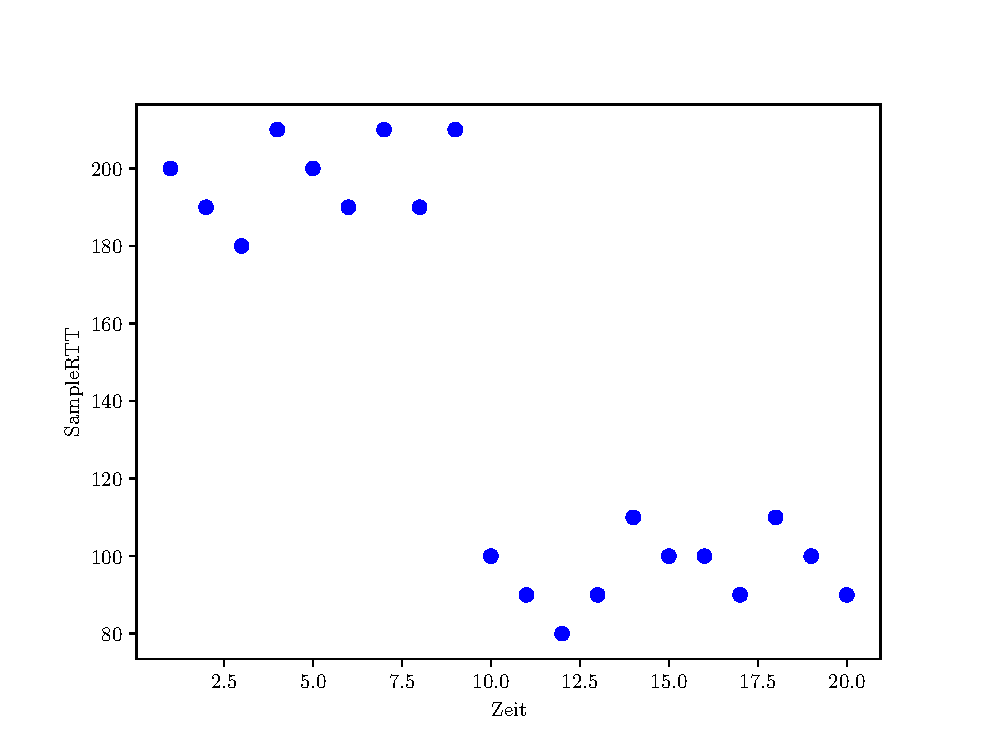
\includegraphics[width=1\textwidth]{./assets/5.12.c.Zeit-SampleRTT.eps}
    \caption{}
    \label{fig:5.12.c.Zeit-SampleRTT}
\end{figure}

\begin{figure}[p]
    \centering
    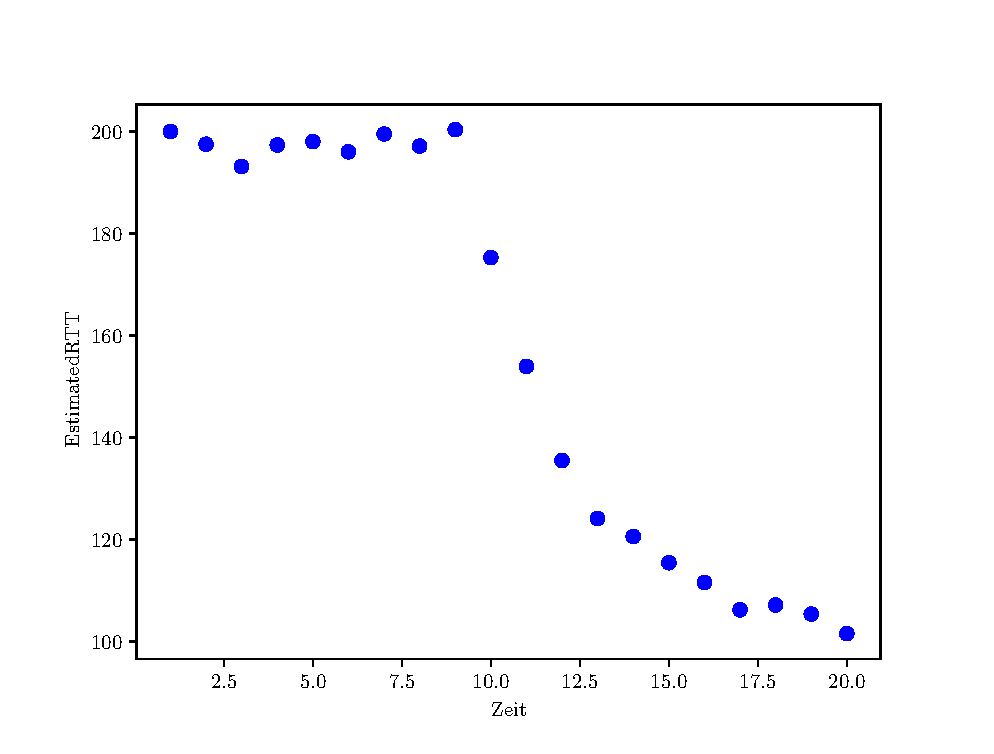
\includegraphics[width=1\textwidth]{./assets/5.12.c.Zeit-EstimatedRTT.eps}
    \caption{}
    \label{fig:5.12.c.Zeit-EstimatedRTT}
\end{figure}

\FloatBarrier

\begin{figure}[p]
    \centering
    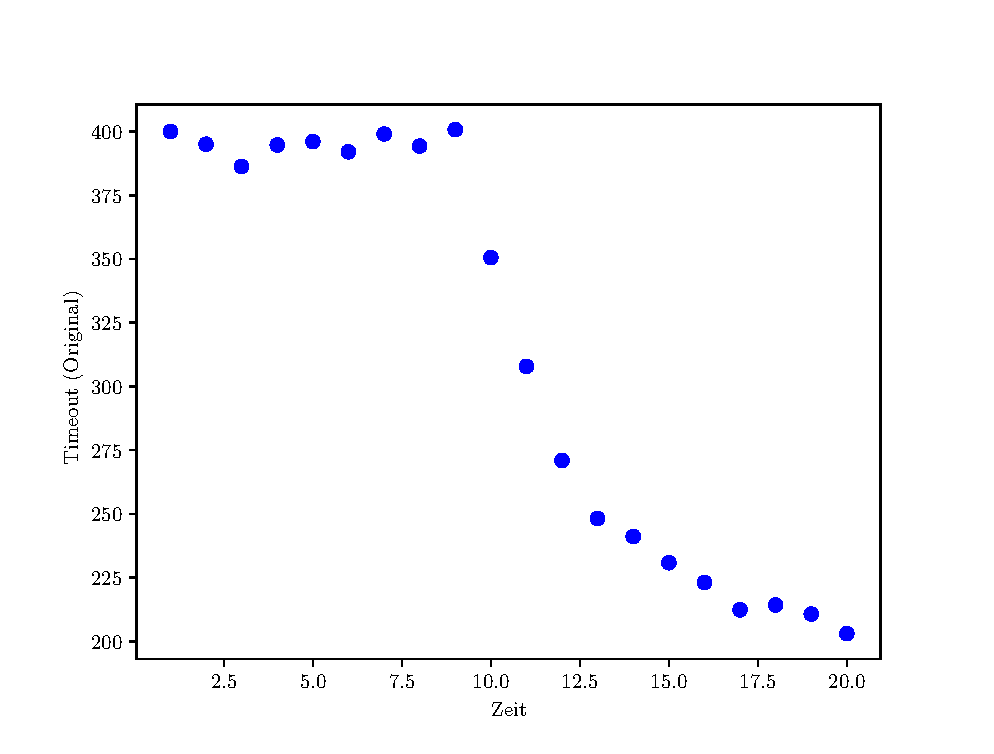
\includegraphics[width=1\textwidth]{./assets/5.12.c.Zeit-Timeout-Original.eps}
    \caption{}
    \label{fig:5.12.c.Zeit-Timeout-Original}
\end{figure}

\begin{figure}[p]
    \centering
    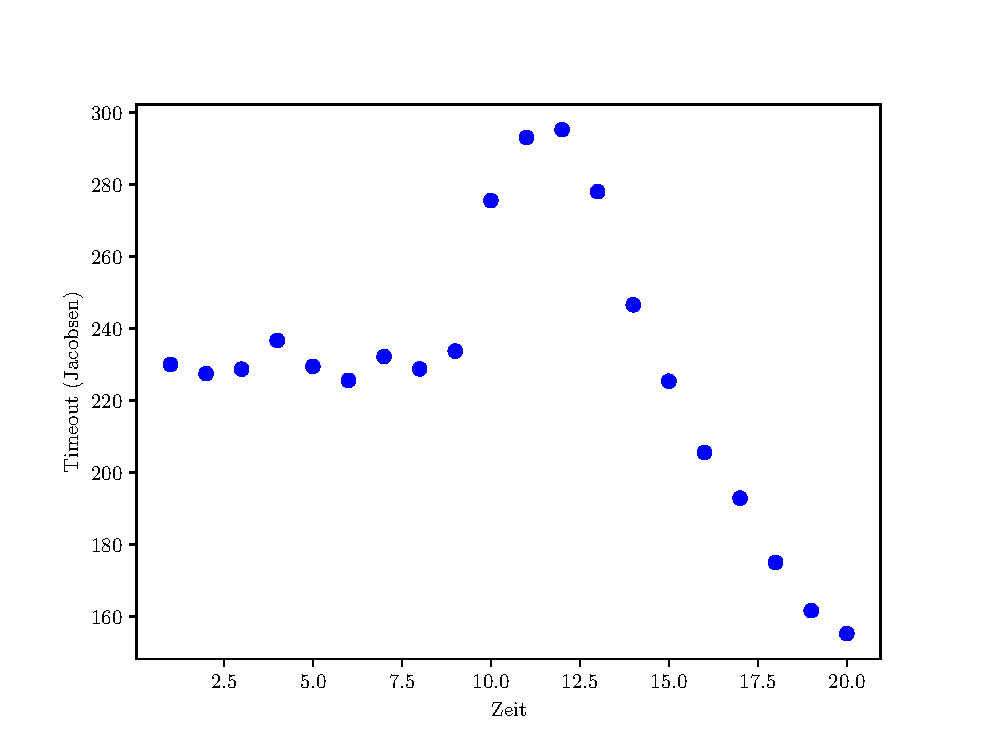
\includegraphics[width=1\textwidth]{./assets/5.12.c.Zeit-Timeout-Jacobsen.eps}
    \caption{}
    \label{fig:5.12.c.Zeit-Timeout-Jacobsen}
\end{figure}

\FloatBarrier
